% Created by tikzDevice version 0.10.1 on 2020-02-15 16:04:59
% !TEX encoding = UTF-8 Unicode
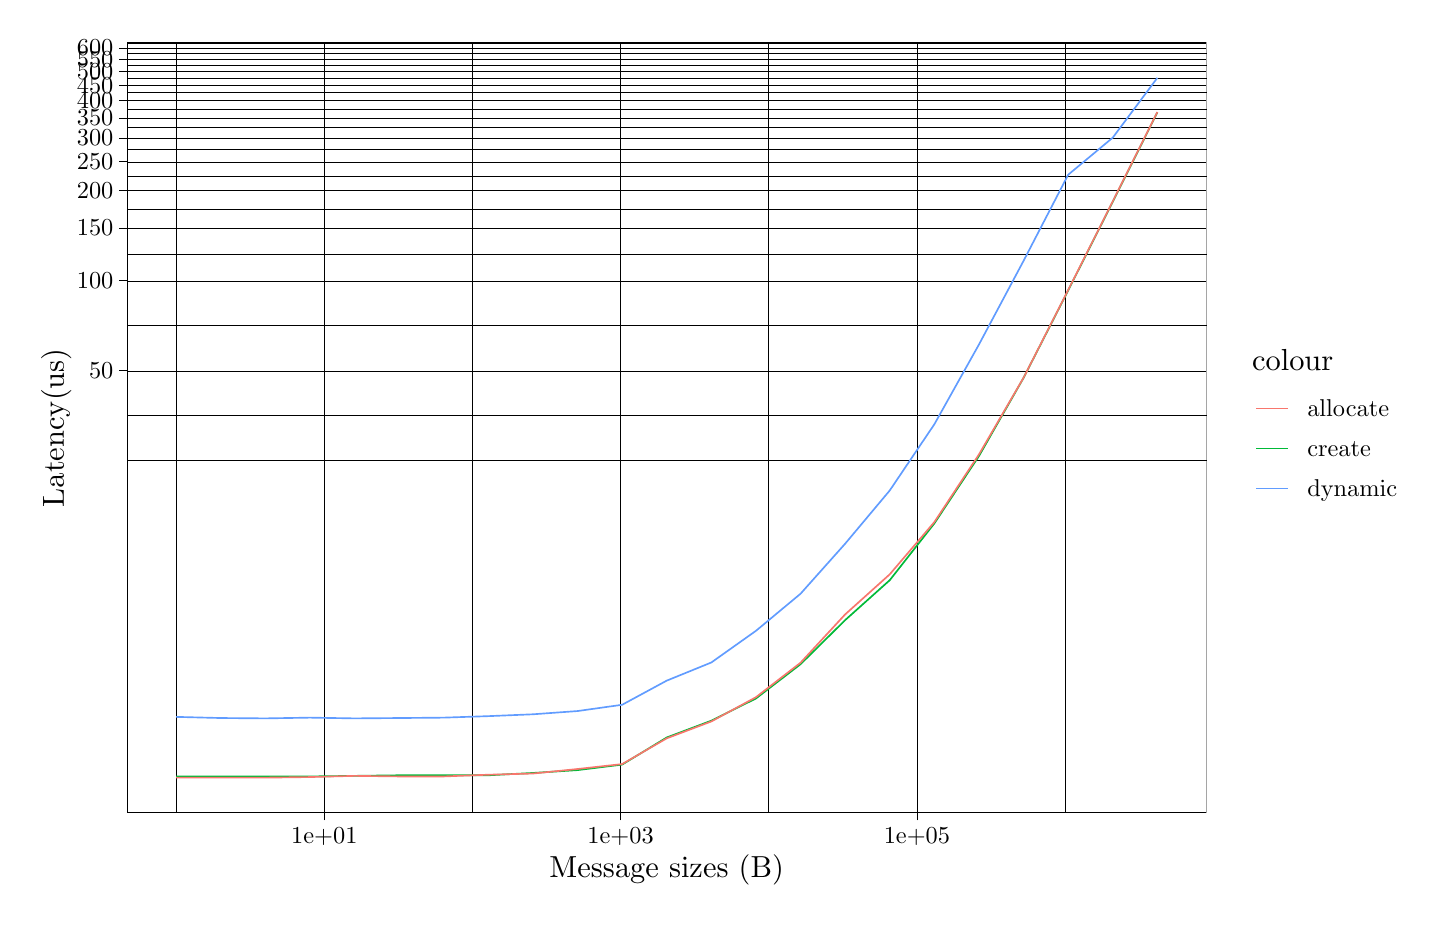
\begin{tikzpicture}[x=1pt,y=1pt]
\definecolor{fillColor}{RGB}{255,255,255}
\path[use as bounding box,fill=fillColor,fill opacity=0.00] (0,0) rectangle (505.89,314.37);
\begin{scope}
\path[clip] (  0.00,  0.00) rectangle (505.89,314.37);
\definecolor{drawColor}{RGB}{255,255,255}
\definecolor{fillColor}{RGB}{255,255,255}

\path[draw=drawColor,line width= 0.6pt,line join=round,line cap=round,fill=fillColor] (  0.00,  0.00) rectangle (505.89,314.37);
\end{scope}
\begin{scope}
\path[clip] ( 35.92, 30.72) rectangle (425.93,308.87);
\definecolor{fillColor}{RGB}{255,255,255}

\path[fill=fillColor] ( 35.92, 30.72) rectangle (425.93,308.87);
\definecolor{drawColor}{RGB}{0,0,0}

\path[draw=drawColor,line width= 0.0pt,line join=round] ( 35.92,157.87) --
	(425.93,157.87);

\path[draw=drawColor,line width= 0.0pt,line join=round] ( 35.92,174.14) --
	(425.93,174.14);

\path[draw=drawColor,line width= 0.0pt,line join=round] ( 35.92,206.68) --
	(425.93,206.68);

\path[draw=drawColor,line width= 0.0pt,line join=round] ( 35.92,232.46) --
	(425.93,232.46);

\path[draw=drawColor,line width= 0.0pt,line join=round] ( 35.92,248.73) --
	(425.93,248.73);

\path[draw=drawColor,line width= 0.0pt,line join=round] ( 35.92,260.71) --
	(425.93,260.71);

\path[draw=drawColor,line width= 0.0pt,line join=round] ( 35.92,270.23) --
	(425.93,270.23);

\path[draw=drawColor,line width= 0.0pt,line join=round] ( 35.92,278.13) --
	(425.93,278.13);

\path[draw=drawColor,line width= 0.0pt,line join=round] ( 35.92,284.88) --
	(425.93,284.88);

\path[draw=drawColor,line width= 0.0pt,line join=round] ( 35.92,290.78) --
	(425.93,290.78);

\path[draw=drawColor,line width= 0.0pt,line join=round] ( 35.92,296.01) --
	(425.93,296.01);

\path[draw=drawColor,line width= 0.0pt,line join=round] ( 35.92,300.72) --
	(425.93,300.72);

\path[draw=drawColor,line width= 0.0pt,line join=round] ( 35.92,305.00) --
	(425.93,305.00);

\path[draw=drawColor,line width= 0.0pt,line join=round] ( 53.64, 30.72) --
	( 53.64,308.87);

\path[draw=drawColor,line width= 0.0pt,line join=round] (160.72, 30.72) --
	(160.72,308.87);

\path[draw=drawColor,line width= 0.0pt,line join=round] (267.79, 30.72) --
	(267.79,308.87);

\path[draw=drawColor,line width= 0.0pt,line join=round] (374.87, 30.72) --
	(374.87,308.87);

\path[draw=drawColor,line width= 0.1pt,line join=round] ( 35.92,190.41) --
	(425.93,190.41);

\path[draw=drawColor,line width= 0.1pt,line join=round] ( 35.92,222.94) --
	(425.93,222.94);

\path[draw=drawColor,line width= 0.1pt,line join=round] ( 35.92,241.97) --
	(425.93,241.97);

\path[draw=drawColor,line width= 0.1pt,line join=round] ( 35.92,255.48) --
	(425.93,255.48);

\path[draw=drawColor,line width= 0.1pt,line join=round] ( 35.92,265.95) --
	(425.93,265.95);

\path[draw=drawColor,line width= 0.1pt,line join=round] ( 35.92,274.51) --
	(425.93,274.51);

\path[draw=drawColor,line width= 0.1pt,line join=round] ( 35.92,281.74) --
	(425.93,281.74);

\path[draw=drawColor,line width= 0.1pt,line join=round] ( 35.92,288.01) --
	(425.93,288.01);

\path[draw=drawColor,line width= 0.1pt,line join=round] ( 35.92,293.54) --
	(425.93,293.54);

\path[draw=drawColor,line width= 0.1pt,line join=round] ( 35.92,298.49) --
	(425.93,298.49);

\path[draw=drawColor,line width= 0.1pt,line join=round] ( 35.92,302.96) --
	(425.93,302.96);

\path[draw=drawColor,line width= 0.1pt,line join=round] ( 35.92,307.04) --
	(425.93,307.04);

\path[draw=drawColor,line width= 0.1pt,line join=round] (107.18, 30.72) --
	(107.18,308.87);

\path[draw=drawColor,line width= 0.1pt,line join=round] (214.26, 30.72) --
	(214.26,308.87);

\path[draw=drawColor,line width= 0.1pt,line join=round] (321.33, 30.72) --
	(321.33,308.87);
\definecolor{drawColor}{RGB}{0,186,56}

\path[draw=drawColor,line width= 0.6pt,line join=round] ( 53.64, 43.80) --
	( 69.76, 43.80) --
	( 85.88, 43.80) --
	(101.99, 43.80) --
	(118.11, 44.01) --
	(134.23, 44.22) --
	(150.34, 44.22) --
	(166.46, 44.22) --
	(182.58, 45.06) --
	(198.69, 46.09) --
	(214.81, 48.08) --
	(230.92, 57.88) --
	(247.04, 63.95) --
	(263.16, 71.97) --
	(279.27, 84.35) --
	(295.39,100.29) --
	(311.51,114.72) --
	(327.62,135.22) --
	(343.74,159.57) --
	(359.86,187.82) --
	(375.97,219.40) --
	(392.09,251.46) --
	(408.20,283.75);
\definecolor{drawColor}{RGB}{248,118,109}

\path[draw=drawColor,line width= 0.6pt,line join=round] ( 53.64, 43.37) --
	( 69.76, 43.37) --
	( 85.88, 43.37) --
	(101.99, 43.58) --
	(118.11, 44.01) --
	(134.23, 43.80) --
	(150.34, 43.80) --
	(166.46, 44.43) --
	(182.58, 44.85) --
	(198.69, 46.49) --
	(214.81, 48.27) --
	(230.92, 57.57) --
	(247.04, 63.67) --
	(263.16, 72.44) --
	(279.27, 84.89) --
	(295.39,102.35) --
	(311.51,116.84) --
	(327.62,135.71) --
	(343.74,160.16) --
	(359.86,187.88) --
	(375.97,219.56) --
	(392.09,251.61) --
	(408.20,283.90);
\definecolor{drawColor}{RGB}{97,156,255}

\path[draw=drawColor,line width= 0.6pt,line join=round] ( 53.64, 65.32) --
	( 69.76, 64.91) --
	( 85.88, 64.78) --
	(101.99, 65.05) --
	(118.11, 64.78) --
	(134.23, 64.91) --
	(150.34, 65.05) --
	(166.46, 65.59) --
	(182.58, 66.26) --
	(198.69, 67.43) --
	(214.81, 69.70) --
	(230.92, 78.42) --
	(247.04, 84.98) --
	(263.16, 96.42) --
	(279.27,109.82) --
	(295.39,127.90) --
	(311.51,147.14) --
	(327.62,171.05) --
	(343.74,199.87) --
	(359.86,230.11) --
	(375.97,261.21) --
	(392.09,274.63) --
	(408.20,296.23);
\definecolor{drawColor}{RGB}{0,0,0}

\path[draw=drawColor,line width= 0.6pt,line join=round,line cap=round] ( 35.92, 30.72) rectangle (425.93,308.87);
\end{scope}
\begin{scope}
\path[clip] (  0.00,  0.00) rectangle (505.89,314.37);
\definecolor{drawColor}{RGB}{0,0,0}

\node[text=drawColor,anchor=base west,inner sep=0pt, outer sep=0pt, scale=  0.88] at ( 22.17,187.59) {50};

\node[text=drawColor,anchor=base west,inner sep=0pt, outer sep=0pt, scale=  0.88] at ( 17.77,220.12) {100};

\node[text=drawColor,anchor=base west,inner sep=0pt, outer sep=0pt, scale=  0.88] at ( 17.77,239.15) {150};

\node[text=drawColor,anchor=base west,inner sep=0pt, outer sep=0pt, scale=  0.88] at ( 17.77,252.66) {200};

\node[text=drawColor,anchor=base west,inner sep=0pt, outer sep=0pt, scale=  0.88] at ( 17.77,263.13) {250};

\node[text=drawColor,anchor=base west,inner sep=0pt, outer sep=0pt, scale=  0.88] at ( 17.77,271.69) {300};

\node[text=drawColor,anchor=base west,inner sep=0pt, outer sep=0pt, scale=  0.88] at ( 17.77,278.92) {350};

\node[text=drawColor,anchor=base west,inner sep=0pt, outer sep=0pt, scale=  0.88] at ( 17.77,285.19) {400};

\node[text=drawColor,anchor=base west,inner sep=0pt, outer sep=0pt, scale=  0.88] at ( 17.77,290.72) {450};

\node[text=drawColor,anchor=base west,inner sep=0pt, outer sep=0pt, scale=  0.88] at ( 17.77,295.66) {500};

\node[text=drawColor,anchor=base west,inner sep=0pt, outer sep=0pt, scale=  0.88] at ( 17.77,300.14) {550};

\node[text=drawColor,anchor=base west,inner sep=0pt, outer sep=0pt, scale=  0.88] at ( 17.77,304.22) {600};
\end{scope}
\begin{scope}
\path[clip] (  0.00,  0.00) rectangle (505.89,314.37);
\definecolor{drawColor}{RGB}{0,0,0}

\path[draw=drawColor,line width= 0.3pt,line join=round] ( 33.17,190.41) --
	( 35.92,190.41);

\path[draw=drawColor,line width= 0.3pt,line join=round] ( 33.17,222.94) --
	( 35.92,222.94);

\path[draw=drawColor,line width= 0.3pt,line join=round] ( 33.17,241.97) --
	( 35.92,241.97);

\path[draw=drawColor,line width= 0.3pt,line join=round] ( 33.17,255.48) --
	( 35.92,255.48);

\path[draw=drawColor,line width= 0.3pt,line join=round] ( 33.17,265.95) --
	( 35.92,265.95);

\path[draw=drawColor,line width= 0.3pt,line join=round] ( 33.17,274.51) --
	( 35.92,274.51);

\path[draw=drawColor,line width= 0.3pt,line join=round] ( 33.17,281.74) --
	( 35.92,281.74);

\path[draw=drawColor,line width= 0.3pt,line join=round] ( 33.17,288.01) --
	( 35.92,288.01);

\path[draw=drawColor,line width= 0.3pt,line join=round] ( 33.17,293.54) --
	( 35.92,293.54);

\path[draw=drawColor,line width= 0.3pt,line join=round] ( 33.17,298.49) --
	( 35.92,298.49);

\path[draw=drawColor,line width= 0.3pt,line join=round] ( 33.17,302.96) --
	( 35.92,302.96);

\path[draw=drawColor,line width= 0.3pt,line join=round] ( 33.17,307.04) --
	( 35.92,307.04);
\end{scope}
\begin{scope}
\path[clip] (  0.00,  0.00) rectangle (505.89,314.37);
\definecolor{drawColor}{RGB}{0,0,0}

\path[draw=drawColor,line width= 0.3pt,line join=round] (107.18, 27.97) --
	(107.18, 30.72);

\path[draw=drawColor,line width= 0.3pt,line join=round] (214.26, 27.97) --
	(214.26, 30.72);

\path[draw=drawColor,line width= 0.3pt,line join=round] (321.33, 27.97) --
	(321.33, 30.72);
\end{scope}
\begin{scope}
\path[clip] (  0.00,  0.00) rectangle (505.89,314.37);
\definecolor{drawColor}{RGB}{0,0,0}

\node[text=drawColor,anchor=base,inner sep=0pt, outer sep=0pt, scale=  0.88] at (107.18, 19.71) {1e+01};

\node[text=drawColor,anchor=base,inner sep=0pt, outer sep=0pt, scale=  0.88] at (214.26, 19.71) {1e+03};

\node[text=drawColor,anchor=base,inner sep=0pt, outer sep=0pt, scale=  0.88] at (321.33, 19.71) {1e+05};
\end{scope}
\begin{scope}
\path[clip] (  0.00,  0.00) rectangle (505.89,314.37);
\definecolor{drawColor}{RGB}{0,0,0}

\node[text=drawColor,anchor=base,inner sep=0pt, outer sep=0pt, scale=  1.10] at (230.92,  7.44) {Message sizes (B)};
\end{scope}
\begin{scope}
\path[clip] (  0.00,  0.00) rectangle (505.89,314.37);
\definecolor{drawColor}{RGB}{0,0,0}

\node[text=drawColor,rotate= 90.00,anchor=base,inner sep=0pt, outer sep=0pt, scale=  1.10] at ( 13.08,169.80) {Latency(us)};
\end{scope}
\begin{scope}
\path[clip] (  0.00,  0.00) rectangle (505.89,314.37);
\definecolor{fillColor}{RGB}{255,255,255}

\path[fill=fillColor] (436.93,135.11) rectangle (500.39,204.49);
\end{scope}
\begin{scope}
\path[clip] (  0.00,  0.00) rectangle (505.89,314.37);
\definecolor{drawColor}{RGB}{0,0,0}

\node[text=drawColor,anchor=base west,inner sep=0pt, outer sep=0pt, scale=  1.10] at (442.43,190.44) {colour};
\end{scope}
\begin{scope}
\path[clip] (  0.00,  0.00) rectangle (505.89,314.37);
\definecolor{fillColor}{RGB}{255,255,255}

\path[fill=fillColor] (442.43,169.52) rectangle (456.89,183.97);
\end{scope}
\begin{scope}
\path[clip] (  0.00,  0.00) rectangle (505.89,314.37);
\definecolor{drawColor}{RGB}{248,118,109}

\path[draw=drawColor,line width= 0.6pt,line join=round] (443.88,176.74) -- (455.44,176.74);
\end{scope}
\begin{scope}
\path[clip] (  0.00,  0.00) rectangle (505.89,314.37);
\definecolor{drawColor}{RGB}{248,118,109}

\path[draw=drawColor,line width= 0.6pt,line join=round] (443.88,176.74) -- (455.44,176.74);
\end{scope}
\begin{scope}
\path[clip] (  0.00,  0.00) rectangle (505.89,314.37);
\definecolor{drawColor}{RGB}{248,118,109}

\path[draw=drawColor,line width= 0.6pt,line join=round] (443.88,176.74) -- (455.44,176.74);
\end{scope}
\begin{scope}
\path[clip] (  0.00,  0.00) rectangle (505.89,314.37);
\definecolor{fillColor}{RGB}{255,255,255}

\path[fill=fillColor] (442.43,155.06) rectangle (456.89,169.52);
\end{scope}
\begin{scope}
\path[clip] (  0.00,  0.00) rectangle (505.89,314.37);
\definecolor{drawColor}{RGB}{0,186,56}

\path[draw=drawColor,line width= 0.6pt,line join=round] (443.88,162.29) -- (455.44,162.29);
\end{scope}
\begin{scope}
\path[clip] (  0.00,  0.00) rectangle (505.89,314.37);
\definecolor{drawColor}{RGB}{0,186,56}

\path[draw=drawColor,line width= 0.6pt,line join=round] (443.88,162.29) -- (455.44,162.29);
\end{scope}
\begin{scope}
\path[clip] (  0.00,  0.00) rectangle (505.89,314.37);
\definecolor{drawColor}{RGB}{0,186,56}

\path[draw=drawColor,line width= 0.6pt,line join=round] (443.88,162.29) -- (455.44,162.29);
\end{scope}
\begin{scope}
\path[clip] (  0.00,  0.00) rectangle (505.89,314.37);
\definecolor{fillColor}{RGB}{255,255,255}

\path[fill=fillColor] (442.43,140.61) rectangle (456.89,155.06);
\end{scope}
\begin{scope}
\path[clip] (  0.00,  0.00) rectangle (505.89,314.37);
\definecolor{drawColor}{RGB}{97,156,255}

\path[draw=drawColor,line width= 0.6pt,line join=round] (443.88,147.84) -- (455.44,147.84);
\end{scope}
\begin{scope}
\path[clip] (  0.00,  0.00) rectangle (505.89,314.37);
\definecolor{drawColor}{RGB}{97,156,255}

\path[draw=drawColor,line width= 0.6pt,line join=round] (443.88,147.84) -- (455.44,147.84);
\end{scope}
\begin{scope}
\path[clip] (  0.00,  0.00) rectangle (505.89,314.37);
\definecolor{drawColor}{RGB}{97,156,255}

\path[draw=drawColor,line width= 0.6pt,line join=round] (443.88,147.84) -- (455.44,147.84);
\end{scope}
\begin{scope}
\path[clip] (  0.00,  0.00) rectangle (505.89,314.37);
\definecolor{drawColor}{RGB}{0,0,0}

\node[text=drawColor,anchor=base west,inner sep=0pt, outer sep=0pt, scale=  0.88] at (462.39,173.71) {allocate};
\end{scope}
\begin{scope}
\path[clip] (  0.00,  0.00) rectangle (505.89,314.37);
\definecolor{drawColor}{RGB}{0,0,0}

\node[text=drawColor,anchor=base west,inner sep=0pt, outer sep=0pt, scale=  0.88] at (462.39,159.26) {create};
\end{scope}
\begin{scope}
\path[clip] (  0.00,  0.00) rectangle (505.89,314.37);
\definecolor{drawColor}{RGB}{0,0,0}

\node[text=drawColor,anchor=base west,inner sep=0pt, outer sep=0pt, scale=  0.88] at (462.39,144.81) {dynamic};
\end{scope}
\end{tikzpicture}
